% This must be in the first 5 lines to tell arXiv to use pdfLaTeX, which is strongly recommended.
\pdfoutput=1
% In particular, the hyperref package requires pdfLaTeX in order to break URLs across lines.

\documentclass[11pt]{article}

% Change "review" to "final" to generate the final (sometimes called camera-ready) version.
% Change to "preprint" to generate a non-anonymous version with page numbers.
\usepackage[final]{acl}

% Standard package includes
\usepackage{times}
\usepackage{latexsym}

% For proper rendering and hyphenation of words containing Latin characters (including in bib files)
\usepackage[T1]{fontenc}
% For Vietnamese characters
% \usepackage[T5]{fontenc}
% See https://www.latex-project.org/help/documentation/encguide.pdf for other character sets

% This assumes your files are encoded as UTF8
\usepackage[utf8]{inputenc}

% This is not strictly necessary, and may be commented out,
% but it will improve the layout of the manuscript,
% and will typically save some space.
\usepackage{microtype}

% This is also not strictly necessary, and may be commented out.
% However, it will improve the aesthetics of text in
% the typewriter font.
\usepackage{inconsolata}

%Including images in your LaTeX document requires adding
%additional package(s)
\usepackage{graphicx}

\usepackage{acronym}
\usepackage[inline]{enumitem}
% MUST BE THE LAST IMPORT
\usepackage{cleveref}

\acrodef{acti}[ACTI]{Automatic Conspiracy Theory Identification}
\acrodef{llm}[LLM]{Large Language Model}

\newcommand{\meta}[1]{{\color{blue}#1}}

% If the title and author information does not fit in the area allocated, uncomment the following
%
%\setlength\titlebox{<dim>}
%
% and set <dim> to something 5cm or larger.

\title{Large Language Models Project \\
Bertinoro International Spring School (BISS) 2024}

% Author information can be set in various styles:
% For several authors from the same institution:
% \author{Martina Baiardi \and Davide Domini \and Nicolas Farabegoli \and Alessandro Petrella \and Gianni Tumedei }
%         Address line \\ ... \\ Address line}
% if the names do not fit well on one line use
%         Author 1 \\ {\bf Author 2} \\ ... \\ {\bf Author n} \\
% For authors from different institutions:
% \author{Author 1 \\ Address line \\  ... \\ Address line
%         \And  ... \And
%         Author n \\ Address line \\ ... \\ Address line}
% To start a separate ``row'' of authors use \AND, as in
% \author{Author 1 \\ Address line \\  ... \\ Address line
%         \AND
%         Author 2 \\ Address line \\ ... \\ Address line \And
%         Author 3 \\ Address line \\ ... \\ Address line}


\author{
  Martina Baiardi \\
  University of Bologna \\
  {\bf m.baiardi@unibo.it} \\ \And
  Davide Domini \\
  University of Bologna \\
  {\bf davide.domini@unibo.it} \\  \And
  Nicolas Farabegoli \\
  University of Bologna \\
  {\bf nicolas.farabegoli@unibo.it} \\  \AND
  Alessandro Petrella\\
  University of Bologna \\
  {\bf alessandro.petrella@unibo.it} \\ \And
  Gianni Tumedei \\
  University of Bologna \\
  {\bf gianni.tumedei2@unibo.it}
}

\begin{document}

\maketitle

\begin{abstract}
Several social network platforms - such as Telegram, 4chan, and Parler - do not employ strong moderation
policies, causing the proliferation of conspiracy theories in many contexts, like COVID-19 or the war
in Ukraine, and thus diffusing dangerous ideas and generating social harm among their communities.
%
In this paper, we present the process to fine-tune two \acp{llm} architectures
on an Italian dataset from an EVALITA challenge, that requires identifying
conspiracy theories in posts coming from Telegram.
%
We provide details about the two adopted architectures, the model configuration and the training
process adopted in our experiments.
%
\meta{Briefly summarise the finding of the experiments}
\end{abstract}

\section{Task description}\label{sec:task-description}
We conducted a comparative study between \emph{Encoder-based} and \emph{Decoder-only} architectures
on the same task.
%
Specifically, we worked on the \emph{\ac{acti}}~\footnote{\url{https://russogiuseppe.github.io/ACTI/}}
task, that requires identifying conspiracy theories coming from lax moderated policies platforms like
Telegram, 4chan, and Parler.
%
We focused on the \emph{Subtask A}, where a system must recognise if a Telegram post is conspiratorial
or not.
%
To be flagged as conspiratorial, a post must:
\begin{enumerate*}[label=(\roman{*})]
  \item express the belief that major events are controlled by and/or manipulated by powerful people protecting their interests; or
  \item interpret events in a way that supports conspiracy theories.
\end{enumerate*}
A sentence is considered conspiratorial even if it shares some claims intended to undermine commonly accepted views on societal issues.

\section{Dataset description}\label{sec:dataset-description}
The dataset for \ac{acti}-A is in CSV format and contains three columns, namely:
\begin{enumerate*}[label=(\roman*)]
  \item \textbf{id}: represents a unique identifier for the post;
  \item \textbf{comment\_text}: contains the raw text written in the post; and
  \item \textbf{conspiratorial}: represents a binary label where 0 indicates that the post is not conspiratorial,
    while 1 indicates conspiratorial content.
\end{enumerate*}
The dataset is split into two separate CSV files: one, meant for the training process, lists
1842 records, while the other includes 460 posts for testing purposes.
%
Notably, since the task was part of a challenge, the second dataset does not contain the
\textbf{conspiratorial} column by default. 
%
Therefore, the test set was initially labelled by computing the encoding of each sentence using an auxiliary LLM, 
and subsequently, a clustering algorithm was employed in the latent space.
%
However, after an analysis, we noticed that several sentences had been mislabeled. 
%
Fortunately, the \ac{acti} team was kind enough to provide the
missing labels upon our request.

\section{Architecture overview}\label{sec:architecture-overview}
To tackle the \ac{acti}-A subtask, we explored two alternative architectures: an encoder-based one, and
a decoder-only one. Both are detailed in this section.

\subsection{Encoder-based}
For the encoder-based architecture, we tried out some variants of BERT \cite{devlin-etal-2019-bert}, pre-trained on different
datasets.

BERT-based classifiers require the pre-processed input text to undergo a tokenization process, where each
sequence of tokens gets also prepended with a \texttt{[CLS]} token, left-padded up to the maximum sequence
length, or truncated down to it if longer.

Passing through BERT's hidden encoding layers, which apply self-attention, tokens are transformed into
contextual embeddings. Notably, we are only interested in the final hidden state corresponding to the
\texttt{[CLS]} token, that contains an aggregate representation of the entire input sequence, and can be
fed to a linear classifier to obtain the probability distribution of the input belonging to one of the
classes (two, in our case). This solution is represented in \meta{TODO Cref figure}.

\subsection{Decoder-only}
We opted for OpenAI GPT-2 \cite{radford2019language} for our decoder-only architecture, testing some variants of the base
model that were specifically tuned for italian corpus.

For the tokenization process, the main differences when compared to the encoder solution are the inverted
padding direction and the absence of the \texttt{[CLS]} token. In fact, due to the auto-regressive nature
of decoder-only models, we use the last token to make the prediction with GPT-2, instead of the first
(\texttt{[CLS]} in BERT).

With GPT-2, the input passes through multiple decoder blocks, each composed by a masked self-attention layer
and a feed-forward neural network. Finally, for sequence classification, a linear layer is added on top of
GPT-2's decoders, with its output dimension equal to the number of labels (two, in our case). An overview
of the whole process is shown in \meta{TODO Cref figure}.

\section{Experimental setup}\label{sec:experimental-setup}

\subsection{Preprocessing}\label{sec:preprocessing}
The preprocessing stage is a fundamental part in preparing the dataset for fine-tune a \ac{llm}.
%
This process ensures that the data is clean, consistent, and in a format suitable for the next stages.
%
The same preprocessing procedure has been applied for both the models taken into account in \Cref{sec:model-config}.
%
In the following,
we report the steps we adopted for the preprocessing stage.

\paragraph{Dataset exploration}
We use Pandas~\cite{reback2020pandas} to build a DataFrame from the CSV dataset files,
for extracting information and data manipulation.

Preliminary,
a dataset exploration is performed to understand the categorical labels' distribution,
and the posts' length provided in the dataset.
%
\Cref{fig:class-frequency} depicts the class distribution for the \emph{training set} (left chart),
and the \emph{test set} (right chart).
%
Notably,
both the classes for the training and test set are well-balanced,
requiring no rebalancing countermeasure.

Another aspect we are interested in is the post length distribution,
since we are limited in the number of token each model can accept.
%
\Cref{fig:words-distribution} shows the distribution of the posts' length divided by training and test set.
%
The two upper charts provide the distribution on the raw post of both the dataset,
while the two lower charts describe the distribution after the cleanup step (that we will discuss in the next paragraph).
%
As can be observed,
the majority of the posts are concentrated in the range $0-500$ words,
meaning that the most of the dataset will not be truncated when input to the model.
%
The posts' cleanup process do not significantly impact the length distribution of the posts in the datasets.

\paragraph{Text cleaning}
To remove noise from the input data,
we processed the raw posts to remove any irrelevant content for the model's fine-tuning.
%
In particular,
we conducted the following operations:
\begin{enumerate*}[label=(\roman{*})]
  \item remove all the extra space;
  \item remove HTML tags and special characters like \texttt{@};
  \item remove all the http link; and
  \item remove all the \texttt{\#} but preserving the text associated to the hashtag.
\end{enumerate*}
Then,
the dataset is updated with the cleaned version of the posts,
preserving the same file structure.


\begin{figure*}
  \centering
  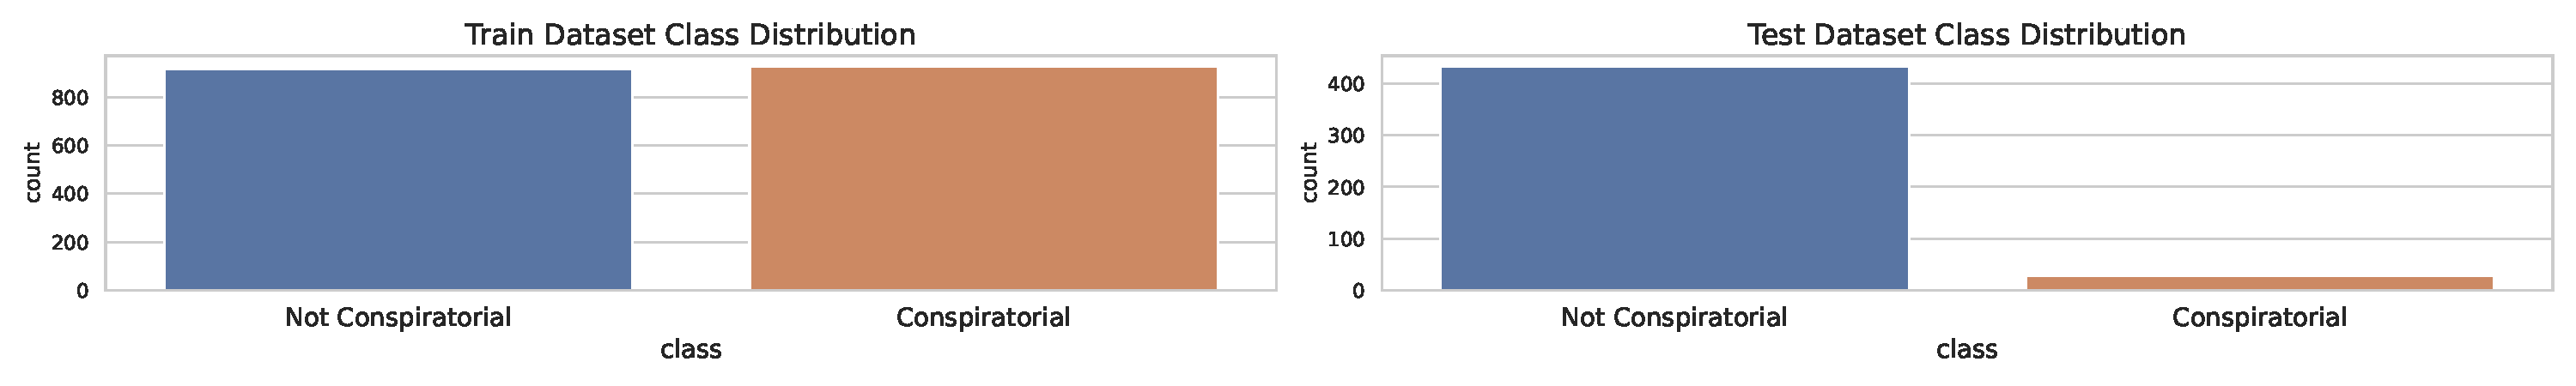
\includegraphics[width=\textwidth]{figures/class_distribution.pdf}
  \caption{
    Class distribution between the \emph{training set} and the \emph{test set}.
  }
  \label{fig:class-frequency}
\end{figure*}

\begin{figure*}
  \centering
  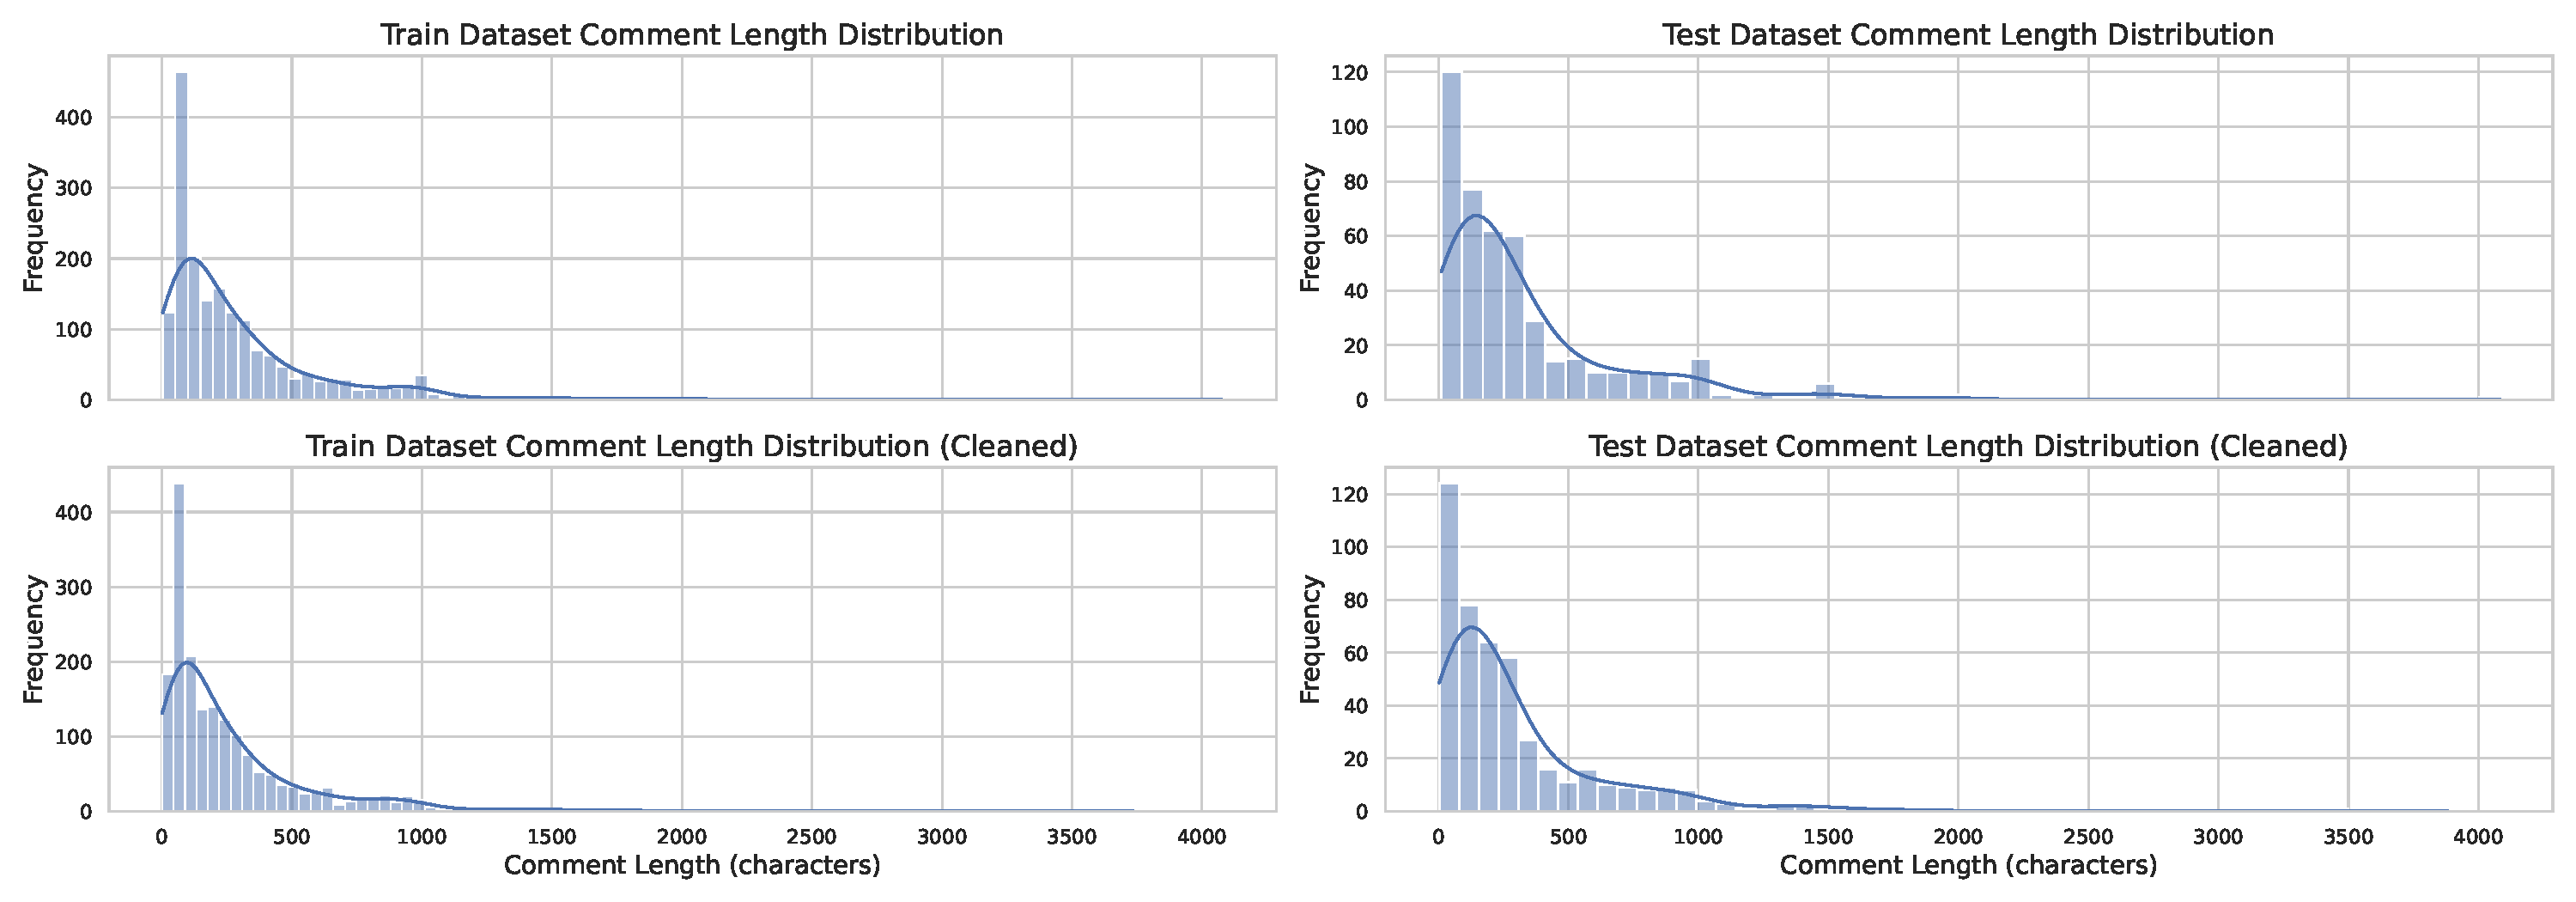
\includegraphics[width=\textwidth]{figures/comment_length_distribution.pdf}
  \caption{
    Comment length distribution for both the training dataset (on the left) and test dataset
    (on the right).
    %
    The upper charts refer to the raw content of posts, coming from the original dataset;
    in the lower charts, our cleanup preprocessing has been applied to the content.
  }
  \label{fig:words-distribution}
\end{figure*}

\subsection{Model configuration}\label{sec:model-config}
%tokenizer, parameters, model used \dots @marti
To solve ACTI-A task, we compared performances of two different Transformer-based architectures,
the first one based on an \emph{Encoder} neural network, and the second one on a \emph{Decoder} neural network.




\subsubsection{Encoder}

% Each BERT-based classifier takes as input a sequence
% of tokens, extracted from the pre-processed text. The
% sequence starts with a classification token [CLS] and is
% concluded by an end-of-sequence token [SEP] , introduced
% during the tokenisation process. To classify the input piece
% of text, we retrieve the contextual embedding computed
% by the transformer hidden layers in correspondence of the
% [CLS] input token and use it to feed a linear classifier. The
% final classification layer outputs the probability distribu-
% tion of the input piece of text to belong to one of the pos-
% sible classes. We reported the entire process in Figure 2a.
% To improve the classification results and take the best
% from the trained models, we considered also creating an
% ensemble [9, Chapter 16]. For each task, we aggregated
% the predictions of the individual models. To aggregate
% the predictions, we froze the fine-tuned classifiers and
% learned a separate Logistic Regression classifier on top
% of the Transformer models. The Logistic Regression
% classifier takes as input the probability distributions
% predicted by individual models and compute a new output
% probability combining the previous. The entire ensemble
% pipeline is represented in Figure 2b

\paragraph{Decoder.}


\subsection{Training process}\label{sec:training-process}
epoche, learning rate, ... @dom

\section{Result and analysis}\label{sec:results-analysis}
@ale
\begin{figure}
  \centering
  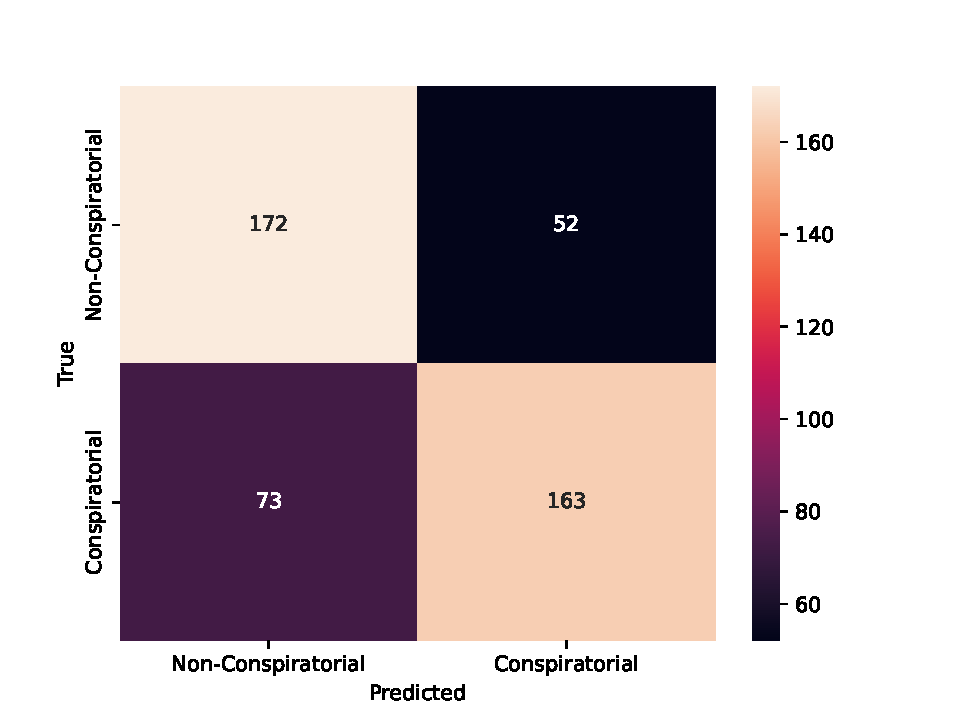
\includegraphics[width=\columnwidth]{figures/decoder-only-confusion-matrix.pdf}
  \caption{
   TBA}
  \label{fig:decoder-only-cm}
\end{figure}

\begin{figure}
  \centering
  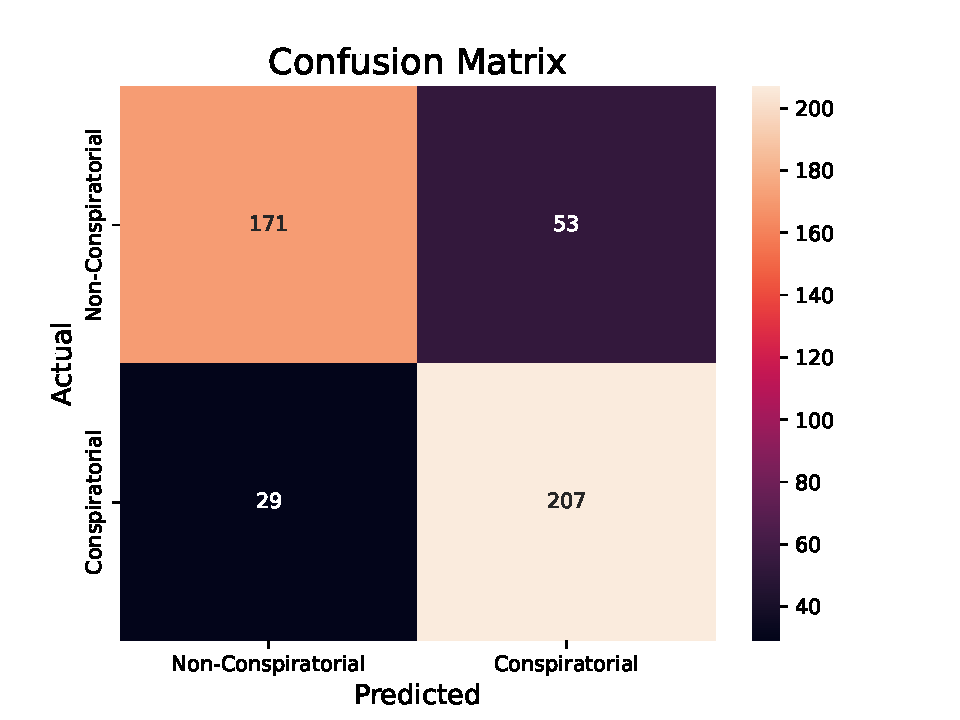
\includegraphics[width=\columnwidth]{figures/encoder-only-confusion-matrix.pdf}
  \caption{
   TBA}
  \label{fig:encoder-only-cm}
\end{figure}


\bibliography{bibliography}

% \appendix

% \section{Example Appendix}
% \label{sec:appendix}

% This is an appendix.

\end{document}
